\subsection{垃圾分类与回收指南}

垃圾分类是法国社会环保和可持续发展的重要组成部分。正确分类和投放垃圾不仅有助于资源回收和环境保护,也是每位居民的法律义务。违规投放可能面临罚款,良好的垃圾分类习惯有助于维护社区环境、促进资源循环利用。

\subsubsection{垃圾分类与投放}
\begin{itemize}
    \item \textbf{可回收垃圾}:包装盒、塑料袋、塑料瓶、金属等散装放入黄色的垃圾桶。玻璃瓶放入玻璃制品特定的垃圾桶。
    \item \textbf{普通垃圾}:无法回收的家庭垃圾,放入密封垃圾袋丢到灰色或棕色垃圾桶。
    \item \textbf{可降解垃圾}:如厨余、果皮、蔬菜残渣、茶叶渣等,可以投入指定的可降解垃圾桶,进而进行堆肥处理。请勿将塑料袋等不可降解物品放入可降解垃圾桶。
    \item \textbf{旧衣物及纺织品}:请投放至专门的旧衣物回收箱(通常分布在小区、超市或市政指定地点),用于再利用或环保处理。
    \item \textbf{有害垃圾}:包括药品、电池、电器、灯管等有害垃圾需要丢弃到专门的回收地点(如药房、指定回收点),请查看居住城市的相关规定。
    \item \textbf{药品}:过期或不用的药品不可随生活垃圾丢弃,应带到药房(Pharmacie)专用回收箱投放,由专业机构统一回收处理,避免环境污染和误用。
    \item \textbf{废旧家具}:请查看居住城市的相关规定,一般情况下每个月或每个礼拜会有固定的时间统一回收。
    \item \textbf{装修垃圾}:需要自行送到垃圾处理厂,请查看居住城市的相关规定。
\end{itemize}

% 图片示例
\begin{figure}[h]
    \centering
    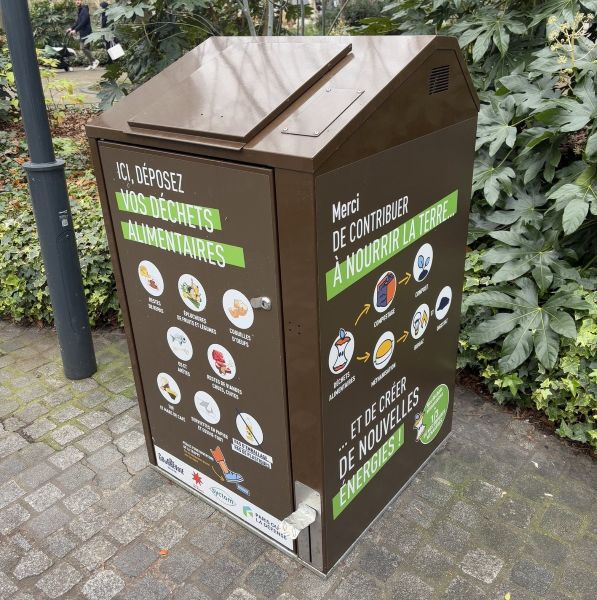
\includegraphics[width=0.4\textwidth]{chapters/06_life/images/garbage_bin_biodegradable.jpg}
    \caption{可降解垃圾桶示意}
\end{figure}

\begin{figure}[h]
    \centering
    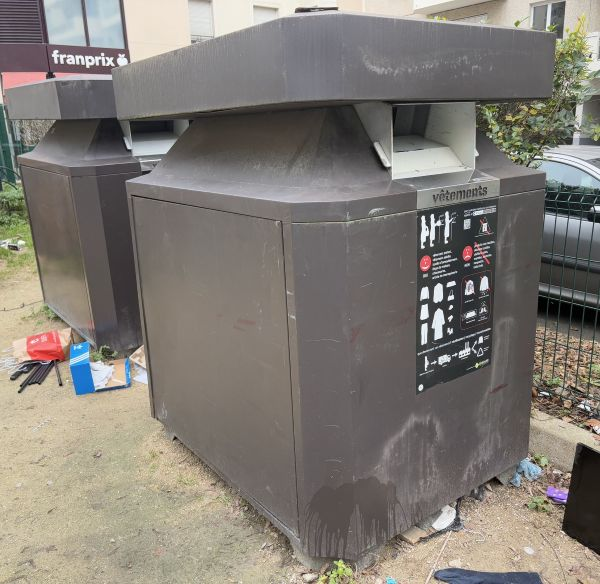
\includegraphics[width=0.4\textwidth]{chapters/06_life/images/garbage_bin_clothes.jpg}
    \caption{衣物回收箱示意}
\end{figure}

\subsubsection{垃圾分类与回收注意事项}
\begin{itemize}
    \item 严格遵守垃圾分类规定,违规投放可能被罚款。
    \item 投放前应清空包装、压缩体积,避免液体泄漏。
    \item 有害垃圾(如电池、药品)切勿与生活垃圾混投。
    \item 关注小区、学校、城市的垃圾回收日程和特殊回收活动。
\end{itemize}

\subsubsection{常用中法垃圾分类词汇}
\begin{itemize}
    \item 垃圾:Déchet
    \item 分类:Tri
    \item 回收:Recyclage
    \item 垃圾桶:Poubelle
    \item 厨余垃圾:Déchets alimentaires
    \item 可回收物:Recyclable
    \item 有害垃圾:Déchets dangereux
    \item 大件垃圾:Encombrants
    \item 回收点:Déchetterie
    \item 药房:Pharmacie
\end{itemize}

